\section{Architecture}
\label{sec:architecture}

\begin{itemize}
  \item Why reactive?
    \url{http://www.reactivemanifesto.org/}
    \begin{figure}[t!]
      \centering
      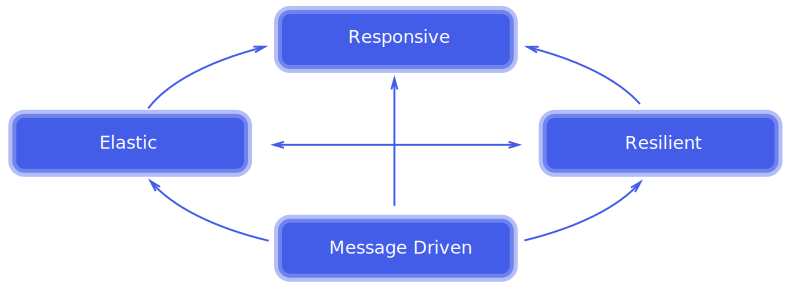
\includegraphics[width=.99\linewidth]{images/reactive-traits}
      \caption{Reactive traits.}
      \label{fig:reactive-traits}
    \end{figure}
  \item Communication by ØMQ (version 4.1.4)
  \item Extension of the library RxLua
  \item Docker container for clustered deployment
  \item Workers connected by routers: define worker's role and router's operating
  \item Fire-and-forget messaging: a messsaging pattern in which we do not expect a direct response to the message, as opposed to request-response protocols
\end{itemize}


\lstset{language=Lua,caption={Descriptive Caption Text},label=DescriptiveLabel}

\begin{lstlisting}[frame=single]
Rx.Observable.fromTable(people)
  :map(
    function(person)
      return person.age
    end
  )
  :filter(
    function(age)
      return age > 18
    end
  )
  :reduce(
    function(accumulator, age)
      accumulator[count] = (accumulator.count or 0) + 1
      accumulator[sum] = (accumulator.sum or 0) + age
      return accumulator
    end, {}
  )
  :subscribe(
    function(datas)
      print('Adult people avverage:', datas.sum / datas.count)
    end,
    function(error)
      print(error)
    end,
    function()
      print('Process complete!')
    end
  )
\end{lstlisting}
